\section{A comparison of races and tournaments in the
field}\label{a-comparison-of-races-and-tournaments-in-the-field}

In this section, we illustrate the preceding econometric methods by an
empirical analysis of the outcomes of a field experiment that was
conducted to compare races and tournaments in the field of online
programming competitions.\footnote{A competitive programming contest is
  a competition that involves participants writing source code for an
  executable computer program to solve a given problem.}

\subsection{The context}\label{the-context}

The study was conducted on the online platform Topcoder.com from March 8
to March 16, 2016. Since its launch in 2010, Topcoder.com hosts on a
weekly basis competitive programming contests for thousands of
competitors from all over the world. All Topcoder members --- about 1M
registered users in 2016 --- can compete and attain a ``rating'' that
provides a metric of their ability as a competitor. Participation is
free but limited to people over 18 years old. Typical assigned problems
are data science problems that involve some background in machine
learning and statistics to be solved (see XXX for a few examples). Other
than attaining a rating, the competitors having made the top five
submissions usually win a monetary prize. And awards can range
considerably depending on the nature and complexity of the problem and
generally between \$5,000 to \$20,000.

\textbf{The assigned problem:} In this study, we worked together with
researchers from the National Health Institute (NIH) and the Scripps
Research Institute to select a challenging problem for an experimental
programming competition. The problem was based on an algorithm built by
NIH that uses expert labeling to annotate abstracts from PubMed --- a
prominent life sciences and biomedical search engine --- so disease
characteristics can be more easily identified. This open-source,
supervised learning system called BANNER achieves a good level of
prediction power {[}see xxx{]}. The goal of the challenge was to improve
upon the current NIH's system.

\textbf{Groups:} Signed up competitors were randomly assigned to
separate groups under three different competitive settings: a race, a
tournament, and a tournament with a minimum quality requirement. Each
group had access to a personalized webpage showing a leaderboard showing
periodic updates on the submissions of the other competitors of the
group.

\textbf{Payoffs:} In each room, the first placed competitor was awarded
a prize of \$1000 (an additional consolatory prize of \$100 was awarded
to the second placed). Every competitor had to solve the same exact
programming problem: it In a race, xxxx. In a tournament, xxxx .And in a
tournament with minimum quality requirement, xxxx.

\textbf{Surveys:} Additional information, such as demographics, all
registered competitors had to fill out online an initial and final
survey before and after the competition. In the initial survey, they
were asked basic demographics, including a measure of risk aversion.
They were also asked to forecast the number of hours they would be able
to spend competing in the next few days. The exact question was:
``looking ahead xxxx''. In the final survey, we asked them to look back
and tell us their best estimate of the time spent working on the
problem.

We also gathered public data from their online web profile on the
platform. This includes a number of statistics about a coder's past
performance on the platoform. We focused on three main measures: the
date in which the member registered, the number of achievements (also
called ``badges''), whether they participated in any similar competition
in the past. The date is simply to capture personal experience with the
platform. Badges are given for a variety of reasons ranging from simple
tasks, such as first post on the forum, to more complex achievements,
such as winning 5 competitions or more. The majority of goals are for
complex achievement, thus having a high number of achievements can be
regarded as a good measure of high skills.

\subsection{Data}\label{data}

A total of 299 competitors signed up for the challenge. All were
registered members of the platform (the competitor's median time as
member of the platform was of 5 years). Individual experience in
competing was highly skewed, with competitors in the 90th percentile
having taken part in 28 more competitions and with a skill rating, if
any, of 999 higher rating points than those in the 10th percentile; see
Figure \ref{eq: distribution experience}.

\begin{figure}
\centering
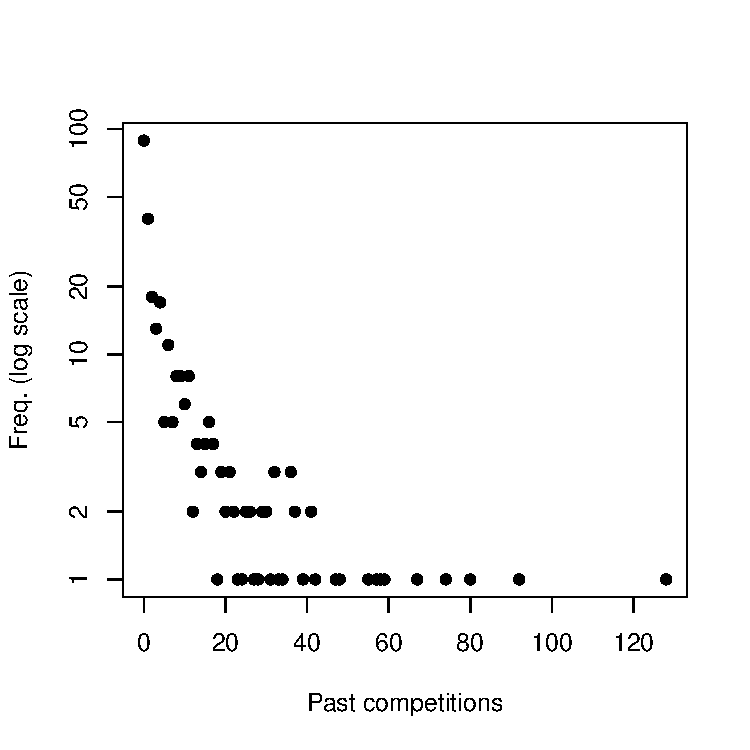
\includegraphics[width=0.45\textwidth]{%
  /Users/andrea/Documents/NTL/races/Workspace/Assets/Figures/experience-1.pdf}
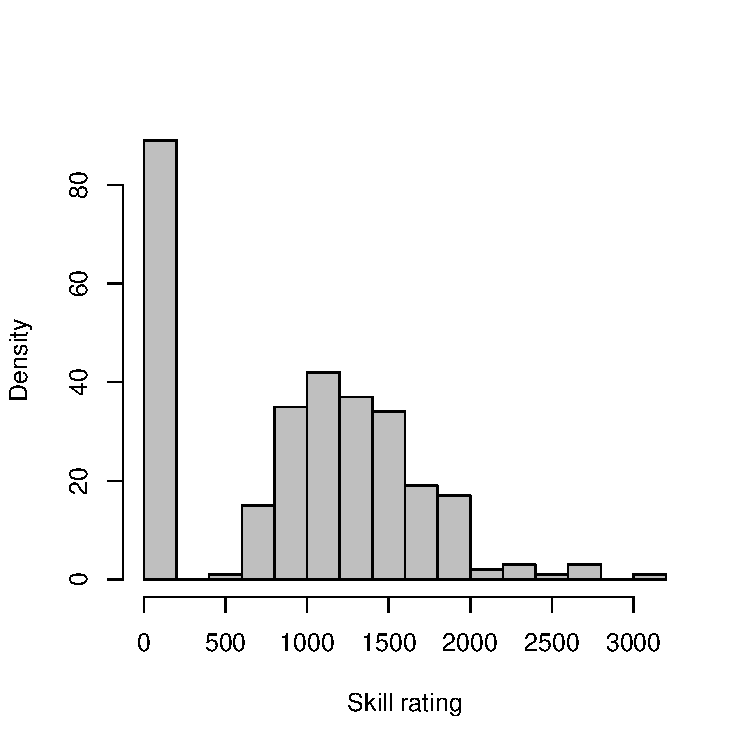
\includegraphics[width=0.45\textwidth]{%
  /Users/andrea/Documents/NTL/races/Workspace/Assets/Figures/rating-1.pdf}
\caption{Distribution of the count of past contests (left panel) and the skill ratings (right panel) of the signed-up competitors.}
\label{eq: distribution experience}
\end{figure}

\section{Empirical analysis}\label{empirical-analysis}

\subsection{Estimation results}\label{estimation-results}

Participation to the competition by treatment is shown in Figure
\ref{fig:entry}. Participation here is measured by the proportion of
registered participants per treatment who made any submission during the
eight-day submission period. Recall that competitors may decide to enter
into the competition and work on the problem without necessarily
submitting. In a tournament, for example, competitors are awarded a
prize based on their last submission and may decide to drop out without
submitting anything. However, this scenario seems unlikely. In fact,
competitors often end up making multiple submissions because by doing so
they obtain intermediate feedback via preliminary scoring (see Section
XXX for details). In a race, competitors have even stronger incentives
to make early submissions as any submission that hits the target first
wins.

\begin{verbatim}
Table xxx
\end{verbatim}

We find that the propensity to make a submission is higher in the
Tournament than in the Race and in the Tournament with reserve, but the
difference is not statistically significant (a Fisher's exact test gives
a p-value of \texttt{r\ round(fisher.test(nsub.tab)\$p.val,3)}). As
discussed in Section XXX, we may not have enough power to detect
differences below 5 percentage points. However, we find the same
not-significant result in a parametric regression analysis of treatment
differences with controls for the demographics and past experience on
the platform; see Table \ref{entry}. Adding individual covariates
reduces variability of outcomes, potentially increasing the power of our
test. In particular, Table \ref{entry} reports the results from a
logistic regression on the probability of making a submissions. Column 1
reports the results from a baseline model with only treatment dummies.
Column 2 adds demographics controls, such as the age, education, and
gender. Column 3 adds controls for the past experience on the platform.
Across all these specifications, the impact of the treatment dummies
(including room size) on entry is not statistically significant.

\subsection{Simulation results}\label{simulation-results}
